\documentclass[11pt]{article}
\usepackage{amsmath,amssymb,amsthm}
\usepackage{graphicx}

\DeclareMathOperator*{\E}{\mathbb{E}}
\let\Pr\relax
\DeclareMathOperator*{\Pr}{\mathbb{P}}

\newcommand{\eps}{\varepsilon}
\newcommand{\inprod}[1]{\left\langle #1 \right\rangle}
\newcommand{\R}{\mathbb{R}}

\newcommand{\handout}[5]{
  \noindent
  \begin{center}
  \framebox{
    \vbox{
      \hbox to 5.78in { {\bf CS 224: Advanced Algorithms } \hfill #2 }
      \vspace{4mm}
      \hbox to 5.78in { {\Large \hfill #5  \hfill} }
      \vspace{2mm}
      \hbox to 5.78in { {\em #3 \hfill #4} }
    }
  }
  \end{center}
  \vspace*{4mm}
}

\newcommand{\lecture}[4]{\handout{#1}{#2}{#3}{Scribe: #4}{Lecture #1}}

\newtheorem{theorem}{Theorem}
\newtheorem{corollary}[theorem]{Corollary}
\newtheorem{lemma}[theorem]{Lemma}
\newtheorem{observation}[theorem]{Observation}
\newtheorem{proposition}[theorem]{Proposition}
\newtheorem{definition}[theorem]{Definition}
\newtheorem{claim}[theorem]{Claim}
\newtheorem{fact}[theorem]{Fact}
\newtheorem{assumption}[theorem]{Assumption}

% 1-inch margins, from fullpage.sty by H.Partl, Version 2, Dec. 15, 1988.
\topmargin 0pt
\advance \topmargin by -\headheight
\advance \topmargin by -\headsep
\textheight 8.9in
\oddsidemargin 0pt
\evensidemargin \oddsidemargin
\marginparwidth 0.5in
\textwidth 6.5in

\parindent 0in
\parskip 1.5ex

\begin{document}

\lecture{15 --- October 21, 2014}{Fall 2014}{Prof.\ Jelani Nelson}{Matt Rauen}

\section{Overview}

In the last lecture we covered nearest neighbor search with guest lecturer Piotr Indyk.

In this lecture we cover solving linear programs using the simplex algorithm.

\begin{enumerate}
\item{Simplex}
\item{Strong duality/complementary slackness}
\item{Ellipsoid}
\end{enumerate}

\section{Standard form}

In a general linear program, we want to minimize $c^Tx$ such that some set of inequalities are satisfied. We would like to convert this into standard form:

$\min c^Tx$ such that $Ax=b$ and $x\ge 0$

$x\in\mathbb{R}^n,A\in\mathbb{R}^{m\times n}, n\ge m$

If we have a maximization problem, we can just flip the sign of $c^T$ and switch it to a minimization problem, since minimizing $-c^Tx$ is equivalent to maximizing $c^Tx$.

\subsection{Getting to standard form}

In order to convert a linear program to standard form, we observe the following two facts:

\begin{fact}
$\langle a_i,x\rangle = b_i\iff \langle a_i,x\rangle \ge b_i\text{ and } -\langle a_i,x\rangle\ge -b_i$
\end{fact}

\begin{fact}
$\langle a_i,x\rangle \le b_i \iff -\langle a_i,x\rangle \ge -b_i$
\end{fact}

Convert all constraints in this way so that we are left with $\ge$ symbols. Then for each constraint $i$, we define a slack variable $s_i\ge 0$ to represent the difference between the sides of the inequality. Replace $\langle a_i,x\rangle \ge b_i$ with $\langle a_i,x\rangle-s_i=b_i$. Then, to account for the constraint that $x\ge 0$, we can write $x_i=x_i^+-x_i^-$ where $x_i^+\ge 0$ and $x_i^-\ge 0$. Note that the number of variables in the new LP is at least the number of constraints, since we are adding a slack variable for each constraint.

\subsection{LPs geometrically}

\begin{center}
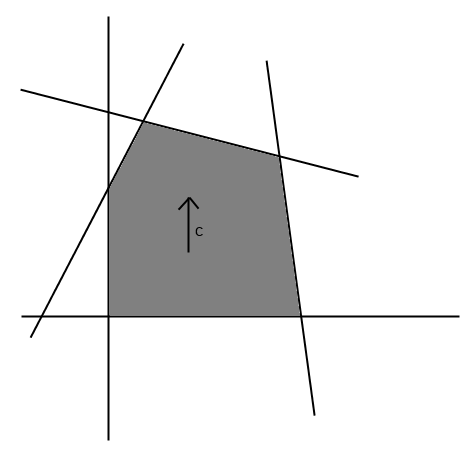
\includegraphics[scale=0.5]{graph.png}
\end{center}

The constraints restrict the region of valid points, and $c$ indicates how the objective function changes with $x$.

\section{Simplex Algorithm}

\underline{Simplex Algorithm} reproduced here \cite{Dantzig47}.

{\bf Main Idea:} Start at some vertex, greedily move to adjacent vertices that improve the objective, and we stop when we are at the optimal vertex.

Let $P=\{x:Ax=b,x\ge 0\}$.

{\bf Definition:} We say that $x\in P$ is a \underline{vertex} if $\nexists y\ne 0$ such that $x-y\in P$ and $x+y\in P$.

We claim that finding an $x$ that satisfies those constraints (that is, lies in $P$) is equivalent to solving the linear program. This is because if we have a guess $r$ for the outcome of the linear program, we can add in the constraint $c^Tx\le r$. Checking if this new LP is satisfiable allows us to bound the minimum, and we can continue via binary search to solve the LP.

This will terminate since the optimal $x$ is a rational number of bounded precision, and our binary search gives you at least a bit of information each time it runs. Here we are operating under the assumptions that the optimal solution is a vertex and that we can obtain the vertices by solving a linear system on $A$, which is what allows us to bound the precision.

Because of this, finding a starting vertex is difficult, so we will run the simplex algorithm on a different LP in order to find one. This other usage of the simplex algorithm has an easy starting vertex, so we only have to run the simplex algorithm twice, once to find the starting vertex, and once to actually solve our LP.

{\bf Starting Vertex LP:} Minimize $t$ such that $Ax=(1-t)b$, $x \ge 0$, and $0\le t \le 1$.

This is not in standard form, since we have the constraint $t\le 1$, but we can rewrite this via a slack variable $s_t$. The constraint becomes $s_t+t=1$ for some $s_t\ge 0$. We have a feasible point given by $x=0$, $t=1$, $s_t=0$.

{\bf Question:} Why is this a vertex?

If $x-y,x+y\in P$, then $y$ cannot have any mass on $x$, since if $y$ or $-y$ is negative on any coordinate corresponding to $x$, we violate $x\ge 0$. It also cannot have any mass on $t$ or $s_t$ since the constraints $t\le 1$ and $s_t\ge 0$ are already tight.

{\bf Definitions:}
\begin{itemize}
\item{$x$ is \underline{feasible} if $x\in P$}
\item{An LP is \underline{feasible} if $\exists$ a feasible $x$}
\item{An LP is \underline{infeasible} if $\nexists$ a feasible $x$}
\item{An LP is \underline{bounded} if $\min c^Tx$ over $x\in P$ is $>-\infty$}
\end{itemize}

{\bf Claim:} If an LP is bounded, then $\forall$ feasible $x$, $\exists$ vertex $x^{\prime}\in P$ such that $c^Tx^{\prime}\le c^Tx$.

\begin{proof}
If $x$ is a vertex, set $x^{\prime}=x$. Else, $\exists y\ne 0$ such that $x+y\in P$ and $x-y\in P$, which implies that $A(x+y)=A(x-y)=b$, so $Ay=0$. Without loss of generality, $c^Ty\le 0$. If this isn't the case, we simply replace $y$ with $-y$. Also, if $c^Ty=0$, then we can assume that there is an index $j$ such that $y_j<0$ (if not, we can just flip the sign of $y$, as before).

{\bf Case 1:} $\exists j$ such that $y_j<0$.

Look at $x+ty$ for $t>0$. If $x_i=0$, then $y_i=0$. If this were not true, then on this coordinate, one of $x+y$ and $x-y$ would violate the constraint that $x\ge 0$. As $t$ increases, $(x+ty)_j$ goes to $0$ for all $j$ such that $y_j<0$.

There is some $t^*>0$ such that $x+t^*y\in P$. Pick $t^*$ as large as possible so that $x+t^*y\in P$.

This case can happen at most $n$ times, since every time it happens, our new $x$ has at least one more coordinate that is $0$. From then on, that coordinate must be fixed so that we don't violate the constraint that $x\ge 0$.

{\bf Question:} Why does a $t^*>0$ exist?

If $y_j<0$ then $x_j> 0$. This implies that $t\cdot y_j+x_j>0$ if $t< -\frac{x_j}{y_j}$. Choose $t^*$ to be the minimum such upper bound over $j$ such that $y_j<0$.

{\bf Case 2:} $\forall j$, $y_j\ge 0$.

Now $A(x+ty)=Ax+t\cdot Ay=b$, and $\forall t > 0$, $x+ty\ge 0$, but $c^T(x+ty)=c^Tx+t\cdot c^Ty<0$ (since otherwise we would be in Case 1). Then $t\to\infty$ demonstrates that the LP is unbounded, which contradicts the assumption that we are in a bounded LP.
\end{proof}

{\bf Corollary:} If an LP is finite, then $\exists$ a vertex in $P$ achieving OPT.

{\bf Corollary:} If $P\ne\emptyset$, then it has at least one vertex.

The second follows from the fact that we can choose any objective function, and then there must be a vertex achieving OPT, so in particular there must be a vertex.

{\bf Definition:} Given $x\in P$, define $A_x$ as the submatrix of $A$ corresponding to $\{j:x_j>0\}=B_x$.

{\bf Claim:} $x$ is a vertex $\iff$ columns of $A_x$ are linearly independent.

Note that the column rank and row rank are both $m$. All redundant rows either make the LP ``infeasible" or are automatically satisfied and can be removed. If we have fewer columns than $m$ in $A_x$, we can pad with more columns to get a square $m\times m$ matrix. 

\begin{proof}
We prove the contrapositive of both directions.

{\bf (i)} $x$ is not a vertex implies that the columns of $A_x$ are linearly dependent.

If $x$ is not a vertex, then $\exists y\ne 0$ such that $x+y,x-y\in P$, which implies that $A_yy=0$, and so $x_i=0\implies y_i=0$. Thus, $A_y$ has dependent columns, and so $A_x$ has dependent columns because $A_y$ is a submatrix of $A_x$.

{\bf (ii)} The columns of $A_x$ being linearly dependent implies that $x$ is not a vertex.

If the columns of $A$ are not linearly independent, then there is some $y\ne 0$ such that $A_xy=0$. We can extend $y$ to $n$ dimensions by making all other coordinates equal to 0. This then implies $\exists y\ne 0$ such that $Ay=0$. For some $t>0$, we have that $x+ty,x-ty\in P$ (since $y$ only has mass in places where $x$ has mass, so we can choose sufficiently small $t$ as we did in our selection of $t^*$). Thus, $x$ is not a vertex.
\end{proof}

\section{Implementation}

For each vertex $x\in P$, we have some basis $B=\{j:x_j>0\}$, and $|B|\le m$. We have the following fact from linear algebra:

\begin{fact}
$Cz, ~C = (C_1,C_2,\ldots,C_m) \implies Cz=\sum_{i=1}^mz_iC_i$.
\end{fact}

Then $Ax=b$ implies that $\sum_ix_iA_i=\sum_{i\in B}x_iA_i=A_Bx_B$. If $|B|=m$, then $A_B$ is $m\times m$ and has full rank, so it is invertible. Thus, $A_Bx_B=b\implies x_B=A_B^{-1}b$. For every vertex $v$, we then extend its base to have size $m$ while still being linearly independent.

Then we can rewrite the LP as $\min c^T_Bx_B+c_N^Tx_N$ where $N=[n]\backslash B$ such that $A_Bx_B+A_Nx_N=b$ and $x_B,x_N\ge 0$. Then for all $x\in P$, we have that $x_B+A_B^{-1}A_Nx_N=A_B^{-1}b$. In particular, $x_B=A_B^{-1}b-A_{B}^{-1}A_Nx_N$, and therefore \begin{align*}
c^Tx &= c_B^Tx_B+c_N^Tx_N \\
{}&= c_B^TA_B^{-1}b-c_B^TA_B^{-1}A_Nx_N+c_N^Tx_N\\
{}&= (c_N-A_N^T(A_B^{-1})^Tc_B)^Tx_N+c_B^TA_B^{-1}b\\
{}&= \tilde{c}^T_Nx_n+c_B^TA_B^{-1}b.
\end{align*}

{\bf Simplex Algorithm:}

\begin{enumerate}
\item{Maintain current vertex $x$ and its base $B$.}
\item{Rewrite LP as above in terms of $x_B,x_n$, etc.}
\item{If $\tilde{c}_N\ge 0$, then HALT and return $x$.}
\item{If $\exists j\in [n]$ such that $\tilde{c}_j<0$, then increment $x_j$ as long as we can so that the feasibility of $x$ is maintained.}
\end{enumerate}

{\bf Annoying Detail:} If we start changing a coordinate in $x_N$, a coordinate in $x_B$ might change, so we change only until some coordinate in $x_B$ hits zero. That is, we keep incrementing $x_j$ as long as $x_B\ge 0$. It might not be possible to increment $x_j$ at all, so we put $j$ into the basis, and evict a coordinate that is already zero. This means that we have reached a new vertex, as a new constraint became tight. Note that it is possible that the ``pivoting rule" that we use to determine which basis element to evict contains a cycle.

There is a pivoting rule which provably has no infinite loops. It is known as Bland's rule, and is proved in \cite{BlandMOR77}. No implementation of the simplex algorithm will run in polynomial time, but they tend to be reasonably fast in practice.

\bibliographystyle{alpha}

\begin{thebibliography}{42}

\bibitem{Dantzig47}
George~Dantzig.
\newblock Maximization of a linear function of variables subject to linear inequalities.
\newblock In {\em The basic George B. Dantzig}.
\newblock ed. by Richard W. Cottle.
\newblock 24--32, Stanford: Stanford University Press, 2003.

\bibitem{BlandMOR77}
Robert~Bland.
\newblock New Finite Pivoting Rules for the Simplex Method.
\newblock {\em Mathematics of Operations Research}, 2(2):103--107, 1977.

\end{thebibliography}

\end{document}11